\documentclass[border=10pt]{standalone}

\usepackage{tikz}
\usepackage{tikzsymbols}
\usetikzlibrary{calc,patterns,shapes.geometric}

\def\centerarc[#1](#2)(#3:#4:#5){\draw[#1] ($(#2)+({#5*cos(#3)},{#5*sin(#3)})$) arc (#3:#4:#5);}

\begin{document}
	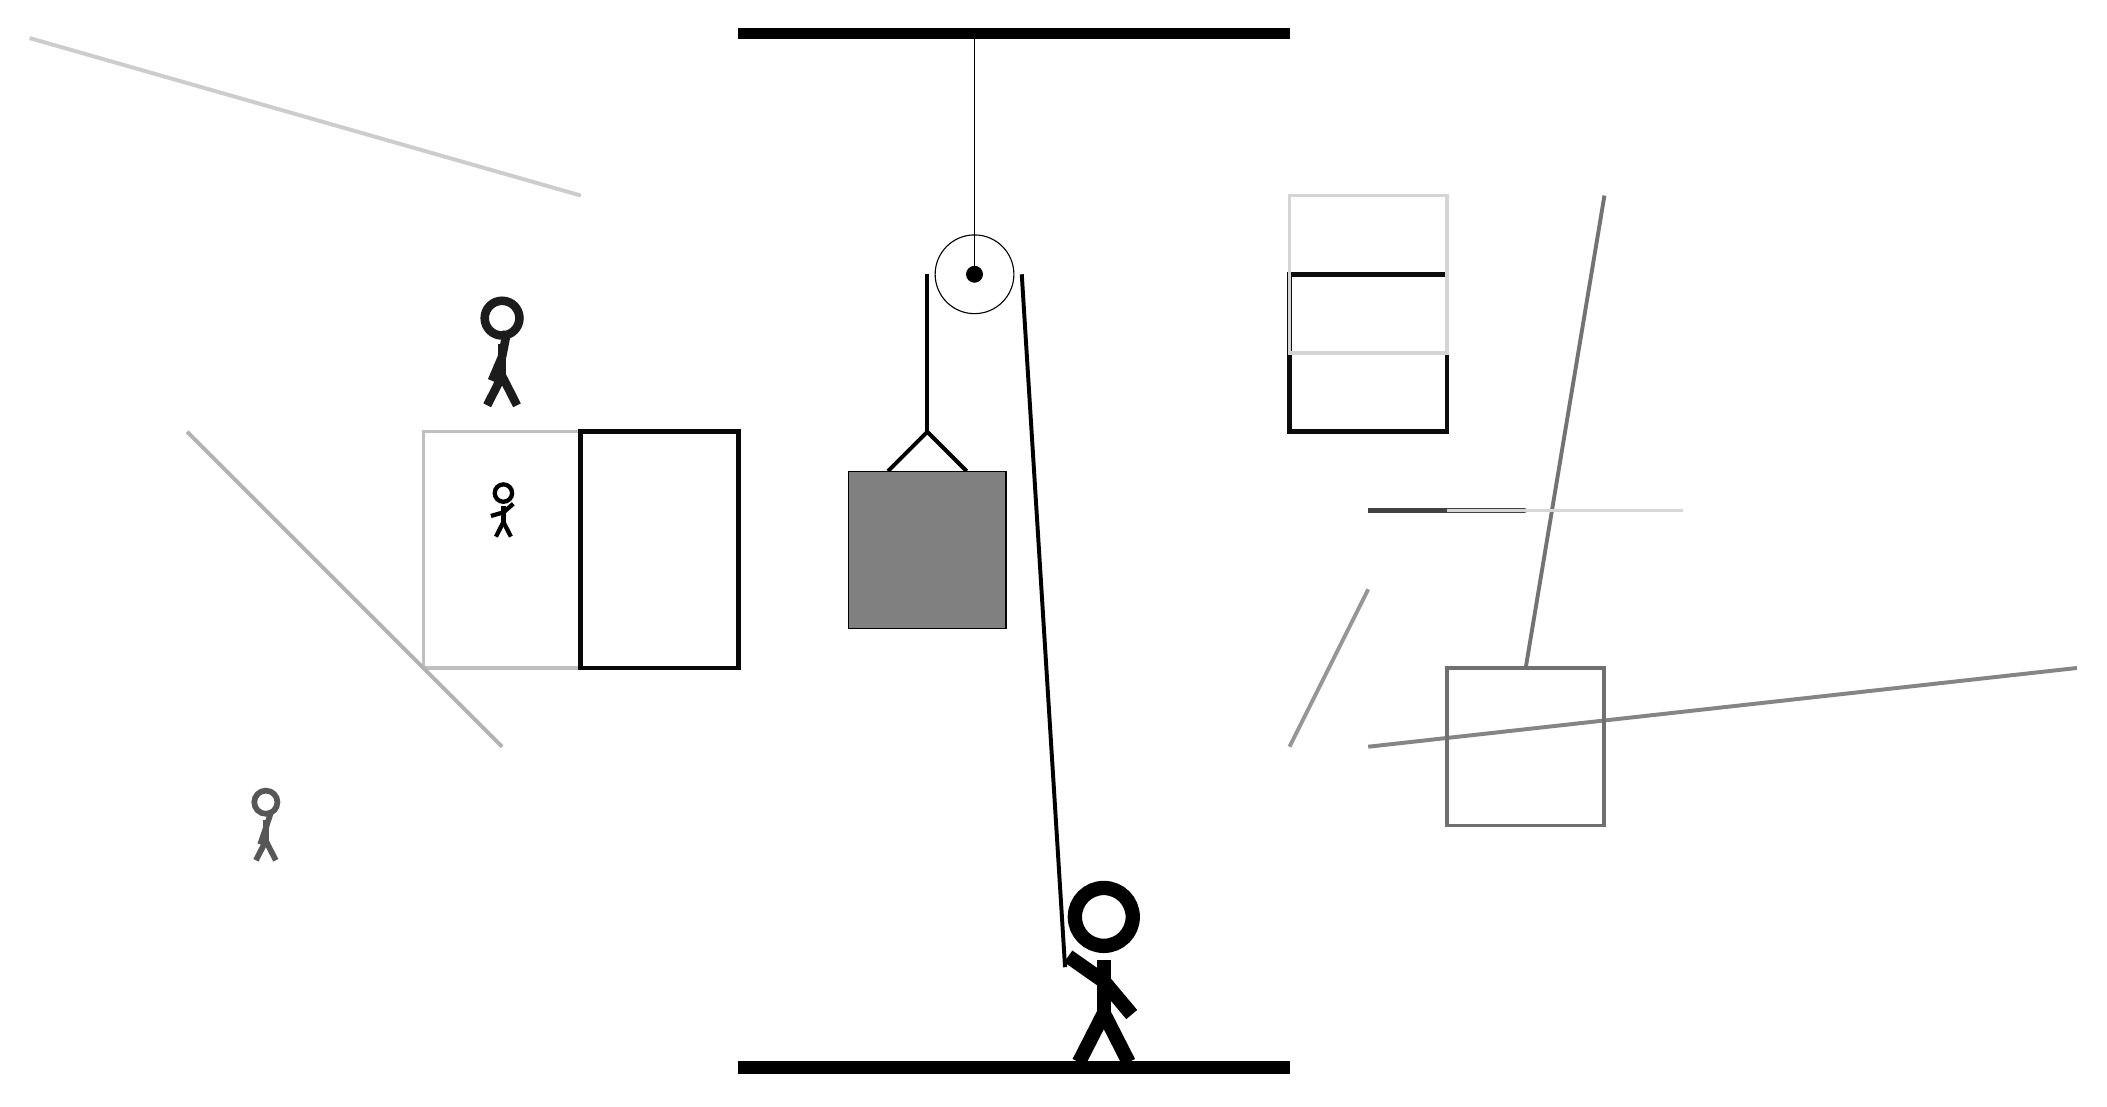
\begin{tikzpicture}
		%%%%% START %%%%%
		
		\draw[fill=black] (-2, 10) rectangle (5, 10.125);
		
		\node[line width=0.6mm, color=black!89] at (-5, 6) {\Strichmaxerl[6][67][79]};
		
		\draw[line width=0.7mm, color=black!74] (6, 4) rectangle (8, 4);
		\draw[line width=0.4mm, color=black!25] (-2, 5) rectangle (-6, 2);
		\node[line width=0.4mm, color=black!66] at (-8, 0) {\Strichmaxerl[4][71][72]};
		\draw[line width=0.5mm, color=black!48](6, 1) -- (15, 2);
		
		\draw[line width=0.5mm, color=black!20](-4, 8) -- (-11, 10);
		\draw[line width=0.6mm, color=black!95] (5, 5) rectangle (7, 7);
		\draw[line width=0.5mm, color=black!41](5, 1) -- (6, 3);
		\draw[line width=0.5mm, color=black!55](8, 2) -- (9, 8);
		
		\draw[line width=0.5mm, color=black!56] (7, 0) rectangle (9, 2);
		\draw[line width=0.5mm, color=black!16](10, 4) -- (7, 4);
		\node[line width=0.7mm, color=black!100] at (-5, 4) {\Strichmaxerl[3][16][41]};
		\draw[line width=0.4mm, color=black!17] (5, 8) rectangle (7, 6);
		
		\draw[line width=0.6mm, color=black!97] (-2, 2) rectangle (-4, 5);
		\draw[line width=0.5mm, color=black!30](-5, 1) -- (-9, 5);
		
		\draw (1, 7) circle (0.5);
		\draw[fill=black] (1, 7) circle (0.1);
		\draw (1, 10) -- (1, 7);
		
		\draw[line width=0.5mm] (-0.1, 4.5) -- (0.4, 5.0) -- (0.9, 4.5);
		\draw[fill=black!50] (-0.6, 4.5) rectangle (1.4, 2.5);
		
		\draw[line width=0.5mm] (0.4, 7) -- (0.4, 5.0);
		\centerarc[line width=0.5mm](1, 7)(0:180:0.6);
		\draw[line width=0.5mm](1.6, 7) -- (2.15, -1.8);
		
		\node at (2.6, -1.9) {\Strichmaxerl[10][-35][-50]};
		
		\draw[fill=black] (-2, -3) rectangle (5, -3.15);
		
		%%%%% END %%%%%
	\end{tikzpicture}
\end{document}